% ==============================================================================
\chapter{Shape Parameterization: Reference Configuration Mapping}
\label{ch:pullback}
% ==============================================================================

To perform shape reduced-order modeling, the governing equations formulated on the parameter-dependent physical domain $\Omega(\boldsymbol{\mu})$ must be mapped to a parameter-independent domain. At the continuum level, this is achieved by defining a smooth, bijective parameterized geometric mapping (diffeomorphism) $\boldsymbol{\Psi}(\cdot; \boldsymbol{\mu}) : \hat{\Omega} \to \Omega(\boldsymbol{\mu})$ that maps any point $\hat{\vect{x}} \in \hat{\Omega}$ in the parameter-independent reference configuration $\hat{\Omega}$ to its counterpart $\vect{x} \in \Omega(\boldsymbol{\mu})$ in the parameterized physical configuration. The overall mapping architecture between the three coordinate domains is illustrated in Figure~\ref{fig:pullback_mapping}.

\begin{figure}[H]
    \centering
    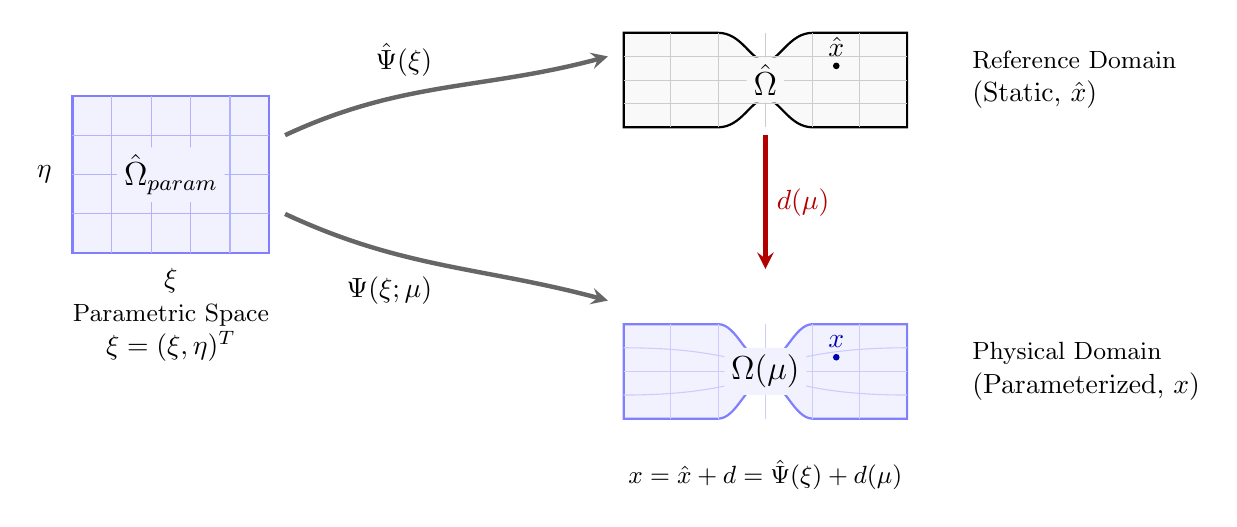
\begin{tikzpicture}[scale=1.0, >=stealth]
        % --- PARAMETRIC DOMAIN (left) ---
        \begin{scope}[xshift=0cm, yshift=0cm]
            \draw[fill=blue!5, draw=blue!50, thick] (0,0) rectangle (2.5,2.0);
            % Grid lines
            \foreach \x in {0.5, 1.0, 1.5, 2.0} {
                \draw[blue!30, thin] (\x, 0) -- (\x, 2.0);
            }
            \foreach \y in {0.5, 1.0, 1.5} {
                \draw[blue!30, thin] (0, \y) -- (2.5, \y);
            }
            % Labels
            \node[below=2pt] at (1.25, 0) {$\xi$};
            \node[left=4pt] at (0, 1.0) {$\eta$};
            \node[fill=blue!5, inner sep=2.5pt, rounded corners=1pt] at (1.25, 1.0) {\large $\hat{\Omega}_{\text{param}}$};
            \node[below=15pt, align=center] at (1.25, 0) {\small Parametric Space \\ $\boldsymbol{\xi} = (\xi, \eta)^T$};
        \end{scope}

        % --- REFERENCE CONFIGURATION (top right) ---
        \begin{scope}[xshift=7.0cm, yshift=2.2cm, scale=0.6]
            % Drawing reference notched beam
            \draw[fill=gray!5, draw=black, thick]
            (0, -1.0) -- (2.0, -1.0)
            .. controls (2.5, -1.0) and (2.7, -0.4) .. (3.0, -0.4)
            .. controls (3.3, -0.4) and (3.5, -1.0) .. (4.0, -1.0)
            -- (6.0, -1.0) -- (6.0, 1.0) -- (4.0, 1.0)
            .. controls (3.5, 1.0) and (3.3, 0.4) .. (3.0, 0.4)
            .. controls (2.7, 0.4) and (2.5, 1.0) .. (2.0, 1.0)
            -- (0, 1.0) -- cycle;
            
            % Grid lines
            \foreach \x in {1, 2, 3, 4, 5} {
                \draw[black!20, thin] (\x, -1.0) -- (\x, 1.0);
            }
            \draw[black!20, thin] (0, -0.5) -- (6.0, -0.5);
            \draw[black!20, thin] (0, 0) -- (6.0, 0);
            \draw[black!20, thin] (0, 0.5) -- (6.0, 0.5);
            
            \fill[black] (4.5, 0.3) circle (2.0pt) node[above] {$\hat{\vect{x}}$};
            \node[fill=gray!5, inner sep=2.5pt, rounded corners=1pt] at (3.0, 0) {\large $\hat{\Omega}$};
            \node[right=20pt, align=left] at (6.0, 0) {\small Reference Domain \\ (Static, $\hat{\vect{x}}$)};
        \end{scope}

        % --- PARAMETERIZED PHYSICAL DOMAIN (bottom right) ---
        \begin{scope}[xshift=7.0cm, yshift=-1.5cm, scale=0.6]
            % Drawing physical notched beam (deeper notches for parameter variation)
            \draw[fill=blue!5, draw=blue!50, thick]
            (0, -1.0) -- (2.0, -1.0)
            .. controls (2.4, -1.0) and (2.6, -0.2) .. (3.0, -0.2)
            .. controls (3.4, -0.2) and (3.6, -1.0) .. (4.0, -1.0)
            -- (6.0, -1.0) -- (6.0, 1.0) -- (4.0, 1.0)
            .. controls (3.6, 1.0) and (3.4, 0.2) .. (3.0, 0.2)
            .. controls (2.6, 0.2) and (2.4, 1.0) .. (2.0, 1.0)
            -- (0, 1.0) -- cycle;
            
            % Grid lines (curved near the notches)
            \foreach \x in {1, 2, 3, 4, 5} {
                \draw[blue!20, thin] (\x, -1.0) -- (\x, 1.0);
            }
            \draw[blue!20, thin] (0, -0.5) .. controls (2, -0.5) and (2.5, -0.15) .. (3.0, -0.15) .. controls (3.5, -0.15) and (4, -0.5) .. (6, -0.5);
            \draw[blue!20, thin] (0, 0) -- (6.0, 0);
            \draw[blue!20, thin] (0, 0.5) .. controls (2, 0.5) and (2.5, 0.15) .. (3.0, 0.15) .. controls (3.5, 0.15) and (4, 0.5) .. (6, 0.5);
            
            \fill[blue!70!black] (4.5, 0.3) circle (2.0pt) node[above] {$\vect{x}$};
            \node[fill=blue!5, inner sep=2.5pt, rounded corners=1pt] at (3.0, 0) {\large $\Omega(\boldsymbol{\mu})$};
            \node[right=20pt, align=left] at (6.0, 0) {\small Physical Domain \\ (Parameterized, $\vect{x}$)};
        \end{scope}

        % --- MAPPING ARROWS ---
        % Parametric to Reference
        \draw[->, ultra thick, black!60] (2.7, 1.5) to[out=25, in=195] node[midway, above left, black] {$\hat{\boldsymbol{\Psi}}(\boldsymbol{\xi})$} (6.8, 2.5);
        
        % Parametric to Physical
        \draw[->, ultra thick, black!60] (2.7, 0.5) to[out=-25, in=165] node[midway, below left, black] {$\boldsymbol{\Psi}(\boldsymbol{\xi}; \boldsymbol{\mu})$} (6.8, -0.6);
        
        % Reference to Physical (Displacement parameterization d(x_c))
        \draw[->, ultra thick, red!70!black] (8.8, 1.5) to[out=-90, in=90] node[midway, right, red!70!black] {$\vect{d}(\boldsymbol{\mu})$} (8.8, -0.2);
        
        % Mathematical relation text
        \node[below, font=\small] at (8.8, -2.5) {$\vect{x} = \hat{\vect{x}} + \vect{d} = \hat{\boldsymbol{\Psi}}(\boldsymbol{\xi}) + \vect{d}(\boldsymbol{\mu})$};
    \end{tikzpicture}
    \caption{Diffeomorphic coordinate mappings between the three domains: the Parametric Space $\hat{\Omega}_{\text{param}}$, the static Reference Domain $\hat{\Omega}$, and the Parameterized Physical Domain $\Omega(\boldsymbol{\mu})$, detailing the pullback relation and parameter-dependent mapping $\vect{d}(\boldsymbol{\mu})$.}
    \label{fig:pullback_mapping}
\end{figure}

This chapter details the mathematical formulation of the pullback at both the continuum and discretized levels, Jacobian transformations, the parameter update mechanism, and compares the naive and reference-pullback paradigms.

\section{Pullback Mapping at the Continuum Level}
The parameterized geometric mapping is defined as:
\begin{equation}
    \vect{x} = \boldsymbol{\Psi}(\hat{\vect{x}}; \boldsymbol{\mu})
\end{equation}
The spatial gradient of this mapping is the coordinate Jacobian matrix $\mathbf{J}_{\hat{\vect{x}}}(\hat{\vect{x}}; \boldsymbol{\mu})$:
\begin{equation}
    \mathbf{J}_{\hat{\vect{x}}}(\hat{\vect{x}}; \boldsymbol{\mu}) = \frac{\partial \boldsymbol{\Psi}(\hat{\vect{x}}; \boldsymbol{\mu})}{\partial \hat{\vect{x}}}
\end{equation}
We assume that the mapping preserves orientation and is invertible, which requires a strictly positive Jacobian determinant:
\begin{equation}
    J_{\hat{\vect{x}}, \boldsymbol{\mu}} = \det \mathbf{J}_{\hat{\vect{x}}}(\hat{\vect{x}}; \boldsymbol{\mu}) > 0 \quad \forall \hat{\vect{x}} \in \hat{\Omega}
\end{equation}
Using the chain rule, the gradients of any physical field $u$ and the differential volume elements are pulled back to the reference configuration via:
\begin{equation}
    \nabla_{\vect{x}} u = \mathbf{J}_{\hat{\vect{x}}}^{-T} \nabla_{\hat{\vect{x}}} \hat{u}, \quad \mathrm{d}\Omega = J_{\hat{\vect{x}}, \boldsymbol{\mu}} \, \mathrm{d}\hat{\Omega}
\end{equation}
where $\hat{u}(\hat{\vect{x}}) = u(\boldsymbol{\Psi}(\hat{\vect{x}}; \boldsymbol{\mu}))$ represents the pulled-back field.

\subsection{Weak Formulation on the Reference Configuration}
By substituting the pullback relations into the variational statement, we project the weak formulation onto the parameter-independent reference configuration $\hat{\Omega}$. The pulled-back weak form reads:
\begin{equation}
    \hat{m}(\ddot{\vect{u}}, \delta\vect{u}; \boldsymbol{\mu}) + \hat{k}(\vect{u}, \delta\vect{u}; \boldsymbol{\mu}) = \hat{f}(\delta\vect{u}) \quad \forall \delta\vect{u} \in \mathcal{V}_0(\hat{\Omega})
\end{equation}
where the mass, stiffness, and load forms are evaluated as integrals over the static reference configuration $\hat{\Omega}$:
\begin{align}
    \hat{m}(\ddot{\vect{u}}, \delta\vect{u}; \boldsymbol{\mu}) & = \int_{\hat{\Omega}} \rho \ddot{\vect{u}} \cdot \delta\vect{u} \, J_{\hat{\vect{x}}, \boldsymbol{\mu}} \, \mathrm{d}\hat{\Omega}                                                                                                                                                 \\
    \hat{k}(\vect{u}, \delta\vect{u}; \boldsymbol{\mu})        & = \int_{\hat{\Omega}} \boldsymbol{\varepsilon}_{\hat{\vect{x}}}(\delta\vect{u})^T \mathbf{J}_{\hat{\vect{x}}}^{-1} \mat{D} \mathbf{J}_{\hat{\vect{x}}}^{-T} \boldsymbol{\varepsilon}_{\hat{\vect{x}}}(\vect{u}) \, J_{\hat{\vect{x}}, \boldsymbol{\mu}} \, \mathrm{d}\hat{\Omega} \\
    \hat{f}(\delta\vect{u})                                    & = \int_{\hat{\Omega}} \vect{f}_b \cdot \delta\vect{u} \, J_{\hat{\vect{x}}, \boldsymbol{\mu}} \, \mathrm{d}\hat{\Omega} + \int_{\hat{\Gamma}_N} \vect{h}_N \cdot \delta\vect{u} \, J_{\hat{\vect{x}}, \boldsymbol{\mu}, \Gamma} \, \mathrm{d}\hat{\Gamma}
\end{align}
Here, $\hat{\Gamma}_N$ represents the reference Neumann boundary, and $J_{\hat{\vect{x}}, \boldsymbol{\mu}, \Gamma}$ is the boundary Jacobian determinant representing the surface area scaling factor. This formulation shifts the entire parameter dependency of the continuum system from the domain geometry into the Jacobian terms $\mathbf{J}_{\hat{\vect{x}}}$ and its determinant $J_{\hat{\vect{x}}, \boldsymbol{\mu}}$.


\section{Diffeomorphic Mapping and Weak Form Pullback in IGA}
The physical domain $\Omega(\boldsymbol{\mu})$ varies with the parameter vector $\boldsymbol{\mu}$, meaning that displacement snapshots collected for different parameters lie in different function spaces. This prevents Proper Orthogonal Decomposition (POD) and SVD-based basis extraction from being conducted directly in the physical space.

To resolve this incompatibility, we define the parameterized smooth geometric mapping (diffeomorphism) $\boldsymbol{\Psi}(\cdot; \boldsymbol{\mu}): \hat{\Omega}_{\text{param}} \to \Omega(\boldsymbol{\mu})$ that maps any parametric point $\boldsymbol{\xi} = (\xi, \eta)^T \in \hat{\Omega}_{\text{param}}$ (where $\boldsymbol{\xi}$ denotes the exact same univariate NURBS parametric coordinates introduced in Chapter~\ref{ch:discretization}) of our parent rectangular parametric configuration to a physical point $\boldsymbol{x} \in \Omega(\boldsymbol{\mu})$:
\begin{equation}
    \boldsymbol{x} = \boldsymbol{\Psi}(\boldsymbol{\xi}; \boldsymbol{\mu}) = \sum_{i=0}^{n-1} \sum_{j=0}^{m-1} R_{i,j}^{p,q}(\boldsymbol{\xi}) \vect{P}_{i,j}(\boldsymbol{\mu})
\end{equation}

The gradient of this mapping is the coordinate Jacobian matrix $\mathbf{J}_{\boldsymbol{\xi}}(\boldsymbol{\xi}; \boldsymbol{\mu})$ defined in Eq.~\eqref{eq:iga_jacobian} of Chapter~\ref{ch:discretization}. We assume that the mapping is bijective and smooth, such that its Jacobian determinant is strictly positive:
\begin{equation}
    J_{\boldsymbol{\xi}, \boldsymbol{\mu}} = \det \mathbf{J}_{\boldsymbol{\xi}}(\boldsymbol{\xi}; \boldsymbol{\mu}) > 0
\end{equation}
By utilizing the pullback relations for spatial gradients and differential volume elements:
\begin{equation}
    \nabla_{\boldsymbol{x}} u = \mathbf{J}_{\boldsymbol{\xi}}^{-T} \nabla_{\boldsymbol{\xi}} \hat{u}, \quad d\Omega = J_{\boldsymbol{\xi}, \boldsymbol{\mu}} \, d\hat{\Omega}_{\text{param}}
\end{equation}
where $\hat{u}(\boldsymbol{\xi}) = u(\boldsymbol{\Psi}(\boldsymbol{\xi}; \boldsymbol{\mu}))$, we transform the integrals in the weak form onto the static reference configuration $\hat{\Omega}$ (or parent parametric space $\hat{\Omega}_{\text{param}}$):
\begin{equation}
    \hat{m}(\ddot{\vect{u}}, \delta\vect{u}; \boldsymbol{\mu}) + \hat{k}(\vect{u}, \delta\vect{u}; \boldsymbol{\mu}) = \hat{f}(\delta\vect{u}; \boldsymbol{\mu}) \quad \forall \delta\vect{u} \in \mathcal{V}_0(\hat{\Omega})
\end{equation}
where the pulled-back bilinear and linear forms are written as:
\begin{align}
    \hat{m}(\ddot{\vect{u}}, \delta\vect{u}; \boldsymbol{\mu}) & = \int_{\hat{\Omega}_{\text{param}}} \rho \ddot{\vect{u}} \cdot \delta\vect{u} \, J_{\boldsymbol{\xi}, \boldsymbol{\mu}} \, d\hat{\Omega}_{\text{param}}                                                                                                                                        \\
    \hat{k}(\vect{u}, \delta\vect{u}; \boldsymbol{\mu})        & = \int_{\hat{\Omega}_{\text{param}}} \hat{\boldsymbol{\varepsilon}}(\delta\vect{u})^T \mat{D} \hat{\boldsymbol{\varepsilon}}(\vect{u}) \, J_{\boldsymbol{\xi}, \boldsymbol{\mu}} \, d\hat{\Omega}_{\text{param}}                                   \\
    \hat{f}(\delta\vect{u}; \boldsymbol{\mu})                       & = \int_{\hat{\Omega}_{\text{param}}} \vect{\hat{f}}_b \cdot \delta\vect{u} \, J_{\boldsymbol{\xi}, \boldsymbol{\mu}} \, d\hat{\Omega}_{\text{param}} + \int_{\hat{\Gamma}_{N,\text{param}}} \vect{\hat{h}}_N \cdot \delta\vect{u} \, J_{\boldsymbol{\xi}, \boldsymbol{\mu}, \Gamma} \, d\hat{\Gamma}_{\text{param}}
\end{align}
In this formulation, all variables are defined over the fixed parametric coordinate space $\boldsymbol{\xi} \in \hat{\Omega}_{\text{param}}$. The dependency on the geometric parameter vector $\boldsymbol{\mu}$ is shifted entirely into the coordinate Jacobian $\mathbf{J}_{\boldsymbol{\xi}}(\boldsymbol{\xi}; \boldsymbol{\mu})$ and its determinant $J_{\boldsymbol{\xi}, \boldsymbol{\mu}}$. This pullback establishes the mathematically consistent framework required to project snapshot states and construct our reduced-order model.

\section{Parameter Update Mechanism and the Naive vs. Pullback Paradigms}
Understanding the computational differences between resolving the governing equations on the parameterized physical domain directly (Naive) versus using the reference configuration mapping (Pullback) is central to shape-parametric Reduced Order Modeling. 

To introduce this concept pedagogically, we distinguish between three distinct spaces and coordinate configurations, as shown schematically in Figure~\ref{fig:pullback_mapping}:
\begin{enumerate}
    \item \textbf{Parametric Space ($\hat{\Omega}_{\text{param}}$)}: The standard flat parent coordinate system $\boldsymbol{\xi} = (\xi, \eta)^T \in [0, 1]^2$ where the univariate NURBS basis functions and element spans are defined.
    \item \textbf{Reference Domain ($\hat{\Omega}$)}: A nominal, parameter-independent configuration of the notched beam where the static coordinates $\hat{\vect{x}}$ are mapped via the fixed geometric function:
          \begin{equation}
              \hat{\vect{x}} = \hat{\boldsymbol{\Psi}}(\boldsymbol{\xi}) = \sum_{i=0}^{n-1} \sum_{j=0}^{m-1} R_{i,j}^{p,q}(\boldsymbol{\xi}) \vect{P}_{i,j}^0
          \end{equation}
          where $\vect{P}_{i,j}^0$ are the nominal coordinates of the control point lattice defining the unnotched rectangular geometry.
    \item \textbf{Parameterized Physical Domain ($\Omega(\boldsymbol{\mu})$)}: The actual coordinate space $\vect{x}$ on which the physical simulation takes place under varying parameters $\boldsymbol{\mu}$. The physical coordinates $\vect{x}$ are represented as a composition of the reference coordinates $\hat{\vect{x}}$ and a parameter-dependent displacement field $\vect{d}(\boldsymbol{\mu})$:
          \begin{equation}
              \vect{x} = \hat{\vect{x}} + \vect{d} = \hat{\boldsymbol{\Psi}}(\boldsymbol{\xi}) + \vect{d}(\boldsymbol{\mu})
          \end{equation}
\end{enumerate}

Based on this decomposition, the two paradigms for shape-parametric simulation differ significantly:
\begin{itemize}
    \item \textbf{The Naive Approach (Physical Domain Simulation)}: In the naive approach, the equations of motion are solved on the physical domain $\Omega(\boldsymbol{\mu})$ directly. As the geometry changes:
          \begin{enumerate}
              \item The mesh must be regenerated for each parameter value $\boldsymbol{\mu}_k$, meaning the number of elements and control points varies, resulting in a vector space size mismatch.
              \item Snapshots collected across different parameter configurations cannot be stored in a single snapshot matrix for Singular Value Decomposition (SVD), rendering POD basis extraction impossible.
              \item The heavy numerical integration and stiffness matrix assembly must be performed online over the physical domain for every parameter change, causing a severe computational bottleneck.
          \end{enumerate}
    \item \textbf{The Pullback Approach (Reference Domain Mapping)}: The pullback approach maps all physical fields to the static reference domain $\hat{\Omega}$. Under this paradigm:
          \begin{enumerate}
              \item The discretization grid and total degrees of freedom remain constant. All snapshot vectors lie in the same vector space, enabling consistent POD basis projection.
              \item The shape parameter changes are captured entirely by updating the coordinate Jacobian matrix $\mat{J}(\boldsymbol{\xi}; \boldsymbol{\mu})$ at the Gauss integration points. The baseline basis functions and element connectivity do not change, making hyper-reduced online updates extremely efficient.
          \end{enumerate}
\end{itemize}

\subsection{Discretization and Algebraic Paradigms}
To clarify how these systems are formed algebraically, we compare the discretization structures resulting from the Naive and Pullback approaches:

\begin{itemize}
    \item \textbf{Naive Discretization (Physical Configuration)}:
          Under the naive approach, the approximation is performed directly on the varying physical domain $\Omega(\boldsymbol{\mu})$. The discretized displacement field $u^h(\boldsymbol{\mu})$ and the virtual displacement field $\delta u^h$ are:
          \begin{equation}
              u^h(\boldsymbol{\mu}) = \sum_{a=0}^{N_{\text{bas}}-1} R_a(\boldsymbol{\mu}) \vect{u}_a(\boldsymbol{\mu}) = \mat{R}(\boldsymbol{\mu}) \vect{U}(\boldsymbol{\mu}), \quad \delta u^h = \mat{R}(\boldsymbol{\mu}) \delta\vect{U}
          \end{equation}
          Because the shape functions $R_a(\boldsymbol{\mu})$ are evaluated on the parameter-dependent configuration, they depend explicitly on $\boldsymbol{\mu}$. Consequently, the stiffness bilinear form $k(u^h, \delta u^h; \boldsymbol{\mu})$ yields a stiffness matrix formulation:
          \begin{equation}
              k(u^h, \delta u^h; \boldsymbol{\mu}) \Rightarrow \delta\vect{U}^T \mat{K}(\boldsymbol{\mu}) \vect{U}
          \end{equation}
          where the changing discretization domain restricts snapshot matrix assembly across parameters.

    \item \textbf{Pullback Discretization (Reference Configuration)}:
          Under the pullback approach, the fields are discretized on the static reference domain $\hat{\Omega}$ using reference coordinates:
          \begin{equation}
              \hat{u}^h(\boldsymbol{\mu}) = \sum_{a=0}^{N_{\text{bas}}-1} \hat{R}_a \hat{\vect{u}}_a(\boldsymbol{\mu}) = \hat{\mat{R}} \hat{\vect{U}}(\boldsymbol{\mu}), \quad \delta\hat{u}^h = \hat{\mat{R}} \delta\hat{\vect{U}}
          \end{equation}
          Here, the reference shape functions $\hat{R}_a$ are evaluated on the flat parametric space $\hat{\Omega}_{\text{param}}$ and do \textbf{not} depend on $\boldsymbol{\mu}$. This is a crucial property: because the basis functions are static, the discretization space is parameter-independent, meaning all snapshot vectors lie in the same vector space. This parameter-independence is the fundamental mathematical property that enables the application of SVD/POD for Reduced Order Modeling.

          The corresponding parameterized bilinear form is:
          \begin{equation}
              \hat{k}(\hat{u}^h, \delta\hat{u}^h; \boldsymbol{\mu}) \Rightarrow \delta\hat{\vect{U}}^T \hat{\mat{K}}(\boldsymbol{\mu}) \hat{\vect{U}}
          \end{equation}
          The shape parameters are updated via the displacement parameterization field:
          \begin{equation}
              \vect{d}(\boldsymbol{\mu}) = \sum_{a=0}^{N_{\text{bas}}-1} \hat{R}_a \vect{d}_a(\boldsymbol{\mu})
          \end{equation}
\end{itemize}
